% !TEX root = technical-report.tex
% !TEX program = xelatex
\documentclass[10pt,a4paper]{article}

\usepackage[a4paper,top=20mm,bottom=22mm,left=19mm,right=19mm,headheight=14pt]{geometry}
\usepackage{fontspec}
\setsansfont{texgyreheros-regular.otf}[BoldFont=texgyreheros-bold.otf,ItalicFont=texgyreheros-italic.otf,BoldItalicFont=texgyreheros-bolditalic.otf]
\setmainfont{texgyreheros-regular.otf}[BoldFont=texgyreheros-bold.otf,ItalicFont=texgyreheros-italic.otf,BoldItalicFont=texgyreheros-bolditalic.otf]
\setmonofont{texgyrecursor-regular.otf}[BoldFont=texgyrecursor-bold.otf,ItalicFont=texgyrecursor-italic.otf,BoldItalicFont=texgyrecursor-bolditalic.otf,Scale=0.88]
\renewcommand{\familydefault}{\sfdefault}
\usepackage{microtype}
\usepackage[table]{xcolor}
\definecolor{GotherBlue}{HTML}{0A84FF}
\definecolor{Ink}{HTML}{111111}
\definecolor{Mid}{HTML}{666666}
\definecolor{Rule}{HTML}{D9DDE3}
\definecolor{Pale}{HTML}{F4F8FC}
\usepackage{titlesec}
\titleformat{\section}{\fontsize{20}{23}\bfseries\color{Ink}}{}{0pt}{}
\titleformat{\subsection}{\fontsize{13.5}{16}\bfseries\color{Ink}}{}{0pt}{}
\titlespacing*{\section}{0pt}{0pt}{12pt}
\titlespacing*{\subsection}{0pt}{16pt}{7pt}
\usepackage{fancyhdr}
\pagestyle{fancy}
\fancyhf{}
\fancyhead[L]{\footnotesize\color{Mid}Göther Labs / Evaluated RTL study}
\fancyhead[R]{\footnotesize\color{Mid}SERV 1.4.0 / VTR 45 nm}
\fancyfoot[L]{\footnotesize\color{Mid}Fixed 64-pair comparison · \EvidenceDate}
\fancyfoot[R]{\footnotesize\color{Mid}\thepage}
\renewcommand{\headrulewidth}{0.4pt}
\renewcommand{\footrulewidth}{0pt}
\usepackage{booktabs,tabularx,array}
\usepackage{siunitx}
\sisetup{detect-all,group-separator={,},group-minimum-digits=4}
\newcolumntype{Y}{>{\rightskip=0pt plus 1fil\relax\arraybackslash}X}
\newcolumntype{R}{>{\raggedleft\arraybackslash}X}
\newcolumntype{P}[1]{>{\rightskip=0pt plus 1fil\relax\arraybackslash}p{#1}}
\newcolumntype{B}[1]{>{\bfseries\rightskip=0pt plus 1fil\relax\arraybackslash}p{#1}}
\usepackage{amsmath,amssymb,mathtools}
\usepackage{enumitem}
\setlist{nosep,leftmargin=5mm}
\usepackage{listings}
\lstdefinelanguage{VerilogDiff}{morekeywords={always,assign,begin,case,default,end,endcase,else,if,module,input,output,reg,wire},sensitive=true,morecomment=[l]{//}}
\lstset{basicstyle=\ttfamily\footnotesize,keywordstyle=\color{GotherBlue}\bfseries,commentstyle=\color{Mid},columns=fullflexible,keepspaces=true,frame=none,backgroundcolor=\color{white},xleftmargin=0pt,aboveskip=7pt,belowskip=7pt,showspaces=false,showtabs=false,showstringspaces=false,breaklines=true,breakatwhitespace=false}
\usepackage{tikz}
\usetikzlibrary{arrows.meta,positioning,calc,fit,backgrounds}
\usepackage{pgfplots}
\pgfplotsset{compat=1.18}
\usepackage[most]{tcolorbox}
\usepackage{hyperref}
\hypersetup{colorlinks=true,linkcolor=Ink,urlcolor=GotherBlue,citecolor=GotherBlue,pdfauthor={Göther Labs},pdftitle={SERV 1.4.0 - fixed 64-pair study with timing regression},pdflang={en-GB}}
\usepackage{seqsplit}

\newcommand{\EvidenceDate}{13 October 2026}
\newcommand{\PairCount}{64}
\newcommand{\CompositeScore}{0.966526}
\newcommand{\CompositeMedian}{0.964972}
\newcommand{\FinalResultHash}{2a39a8c018d80203413dc669316c185fc12a2e085e22f89f001a285d565999b4}
\newcommand{\BaselineRtlHash}{29b5ea77526b3b972ba99c8702524e87035e5a921db6f1a59bb822599203ba91}
\newcommand{\OptimizedRtlHash}{b25b924a34318591d7cfec7097fc5d265a372316757893b2d51a095c5ba01fbe}
\newcommand{\UpperOneSidedScore}{0.967808}
\newcommand{\DelayLowerOneSidedRatio}{1.012620}
\newcommand{\AreaImprovement}{5.8985}
\newcommand{\AreaLow}{5.8305}
\newcommand{\AreaHigh}{5.9664}
\newcommand{\AreaWins}{64}
\newcommand{\AreaTies}{0}
\newcommand{\AreaLosses}{0}
\newcommand{\DelayImprovement}{-1.9478}
\newcommand{\DelayLow}{-2.7749}
\newcommand{\DelayHigh}{-1.1274}
\newcommand{\DelayWins}{16}
\newcommand{\DelayTies}{0}
\newcommand{\DelayLosses}{48}
\newcommand{\PowerImprovement}{5.8835}
\newcommand{\PowerLow}{5.2187}
\newcommand{\PowerHigh}{6.5435}
\newcommand{\PowerWins}{63}
\newcommand{\PowerTies}{0}
\newcommand{\PowerLosses}{1}
\newcommand{\CompositeImprovement}{3.3474}
\newcommand{\CompositeLow}{3.1940}
\newcommand{\CompositeHigh}{3.5006}
\newcommand{\CompositeWins}{64}
\newcommand{\CompositeTies}{0}
\newcommand{\CompositeLosses}{0}
\newcommand{\DelayIncrease}{1.9478}
\newcommand{\DelayIncreaseLow}{1.1274}
\newcommand{\DelayIncreaseHigh}{2.7749}
\newcommand{\BaselineArea}{2,743,359}
\newcommand{\BaselineDelay}{4.220536}
\newcommand{\BaselinePower}{3.577346}
\newcommand{\BaselineFmax}{236.9368}
\newcommand{\OptimizedArea}{2,581,543}
\newcommand{\OptimizedDelay}{4.302744}
\newcommand{\OptimizedPower}{3.366874}
\newcommand{\OptimizedFmax}{232.4098}
\newcommand{\FmaxReduction}{1.9106}
\newcommand{\CloudMin}{-15}
\newcommand{\CloudMax}{20}


\setlength{\parindent}{0pt}
\setlength{\parskip}{5.5pt}
\setlength{\emergencystretch}{2em}
\newcommand{\hash}[1]{{\scriptsize\ttfamily\seqsplit{#1}}}
\newcommand{\better}{\textcolor{GotherBlue}{\textbf{better}}}
\newcommand{\neutral}{\textcolor{Mid}{\textbf{neutral}}}
\newcommand{\smallcaps}[1]{\textcolor{Mid}{\fontsize{8.5}{10}\selectfont\bfseries\MakeUppercase{#1}}}
\newcommand{\newpageheading}[2]{\clearpage\section{#1}\smallcaps{#2}\par\vspace{6pt}}
\newcommand{\yes}{\textcolor{GotherBlue}{\textbf{PASS}}}
\newcommand{\thead}[1]{\textcolor{white}{\textbf{#1}}}

\newtcolorbox{claimbox}[1][]{enhanced,breakable,boxrule=0.6pt,leftrule=2.8pt,colback=white,colframe=GotherBlue,arc=0pt,left=4.5mm,right=4.5mm,top=4mm,bottom=4mm,before upper=\raggedright,#1}
\newtcolorbox{scopebox}[1][]{enhanced,breakable,boxrule=0.5pt,colback=Pale,colframe=Rule,arc=2mm,left=4mm,right=4mm,top=3mm,bottom=3mm,#1}

\tikzset{
  signal/.style={-Latex,draw=Mid,line width=.75pt},
  gate/.style={draw=Rule,fill=white,rounded corners=1.5pt,minimum width=17mm,minimum height=8mm,font=\scriptsize\bfseries,align=center},
  accepted/.style={gate,draw=GotherBlue},
  input/.style={draw=Rule,fill=white,rounded corners=1.5pt,minimum width=10mm,minimum height=7mm,font=\scriptsize,align=center},
}

\definecolor{Regress}{HTML}{B42318}
\newcommand{\worse}{\textcolor{Regress}{\textbf{regression}}}

\begin{document}

% Page 1: portfolio cover.
\thispagestyle{empty}
\begin{tikzpicture}[remember picture,overlay]
  \fill[GotherBlue] (current page.north west) rectangle ([xshift=7mm]current page.south west);
\end{tikzpicture}
\vspace*{43mm}
{\color{Mid}\fontsize{11}{14}\selectfont Göther Labs / Evaluated RTL study}\par
\vspace{5mm}
{\color{Ink}\fontsize{29}{33}\selectfont\bfseries SERV 1.4.0 RTL optimization\\on VTR}\par
\vspace{5mm}
{\color{Mid}\fontsize{13}{16}\selectfont Fixed 64-pair comparison · open 45 nm FPGA proxy}\par
\vspace{17mm}
\begin{claimbox}
{\fontsize{15}{19}\selectfont\bfseries The composite PPA estimate improves by \CompositeImprovement\%, with lower area and power.}\par
\vspace{3mm}
{\color{Regress}\fontsize{14}{18}\selectfont\bfseries Critical-path delay increases by \DelayIncrease\%: the candidate fails the no-regression acceptance rule.}
\end{claimbox}
\vspace{23mm}
{\color{Mid}\fontsize{12}{15}\selectfont Prepared by Göther Labs}\par
\vspace{4mm}
{\color{Mid}\fontsize{12}{15}\selectfont Measurement completed: \EvidenceDate}\par
\vspace{4mm}
{\color{Mid}\fontsize{11}{14}\selectfont 64 complete pairs / 128 implementations · local review edition}\par
\vfill
{\color{Mid}\footnotesize Academic implementation estimates. Not measured silicon, ASIC signoff, commercial-FPGA characterization or measured energy. The separate 12-pair certification sample is unused; project-contract acceptance is not achieved.}\par

% Page 2.
\newpageheading{1. Executive result}{Frozen baseline versus measured candidate}
\begin{claimbox}
\textbf{The equal-weight area-delay-power score improves by \CompositeImprovement\% (two-sided 95\% CI: \CompositeLow\% to \CompositeHigh\%). Delay regresses by \DelayIncrease\% (95\% CI: \DelayIncreaseLow\% to \DelayIncreaseHigh\% higher). This is a measured trade-off, not an accepted portfolio result.}
\end{claimbox}
\renewcommand{\arraystretch}{1.38}
\vspace{2mm}
{\small\rowcolors{2}{Pale}{white}
\begin{tabularx}{\textwidth}{@{}P{24mm}P{29mm}P{29mm}P{25mm}Y@{}}
\rowcolor{Ink}\thead{Metric} & \thead{Baseline aggregate} & \thead{Candidate aggregate} & \thead{Paired change} & \thead{95\% CI / state} \\
Area & \BaselineArea\ MWTA & \OptimizedArea\ MWTA & \AreaImprovement\% lower & \AreaLow\% to \AreaHigh\% lower · \better \\
Critical path & \BaselineDelay\ ns & \OptimizedDelay\ ns & \textcolor{Regress}{\DelayIncrease\% higher} & \DelayIncreaseLow\% to \DelayIncreaseHigh\% higher · \worse \\
Active power & \BaselinePower\ mW & \OptimizedPower\ mW & \PowerImprovement\% lower & \PowerLow\% to \PowerHigh\% lower · \better \\
Composite & 1.000000 & \CompositeScore & \CompositeImprovement\% lower & \CompositeLow\% to \CompositeHigh\% lower · \better \\
\end{tabularx}\rowcolors{2}{}{}
}
\par
\vspace{4mm}
{\large\bfseries Paired primary PPA change}\par
{\small\color{Mid}64 fixed pairs · positive is improvement · bars are two-sided 95\% intervals}\par
\begin{center}\begin{tikzpicture}
\begin{axis}[width=.96\textwidth,height=65mm,ymin=-4,ymax=8,xmin=.6,xmax=4.4,
 xtick={1,2,3,4},xticklabels={Area,Timing,Active power,Composite},
 ytick={-4,-2,0,2,4,6,8},yticklabel={\pgfmathprintnumber{\tick}\%},
 grid=major,grid style={draw=Rule},axis line style={draw=Mid},tick label style={font=\footnotesize},
 ylabel={Improvement versus baseline}]
\addplot[draw=none,fill=Rule,opacity=.55] coordinates {(.6,-.10) (4.4,-.10) (4.4,.10) (.6,.10)} \closedcycle;
\addplot[GotherBlue,line width=1.25pt,mark=*,error bars/.cd,y dir=both,y explicit]
 table[x=x,y=estimate,y error plus=plus,y error minus=minus,col sep=comma]{generated/executive-ci.csv};
\addplot[Regress,only marks,mark=*,mark size=2.5pt,restrict x to domain=1.9:2.1,error bars/.cd,y dir=both,y explicit]
 table[x=x,y=estimate,y error plus=plus,y error minus=minus,col sep=comma]{generated/executive-ci.csv};
\end{axis}\end{tikzpicture}\end{center}
All absolute aggregates are geometric means. The score equally weights paired log area, delay and power ratios. Its median per-pair ratio is \CompositeMedian; that median is not the acceptance estimator. Area wins in 64 pairs, power in 63 and delay in only 16. The composite wins in all 64.

% Page 3.
\newpageheading{2. Processor, boundary and capacity}{What is actually being optimized}
SERV is a bit-serial 32-bit RISC-V processor. The evaluated artifact is the complete eighteen-file RTL tree at SERV tag \texttt{1.4.0}, commit \texttt{7d9cde4e...}, under ISC terms. Each baseline file matches its upstream Git blob byte for byte. The measurement top is \texttt{serv\_synth\_wrapper}; it includes the CPU and register-file interface but leaves register storage external.

\begin{center}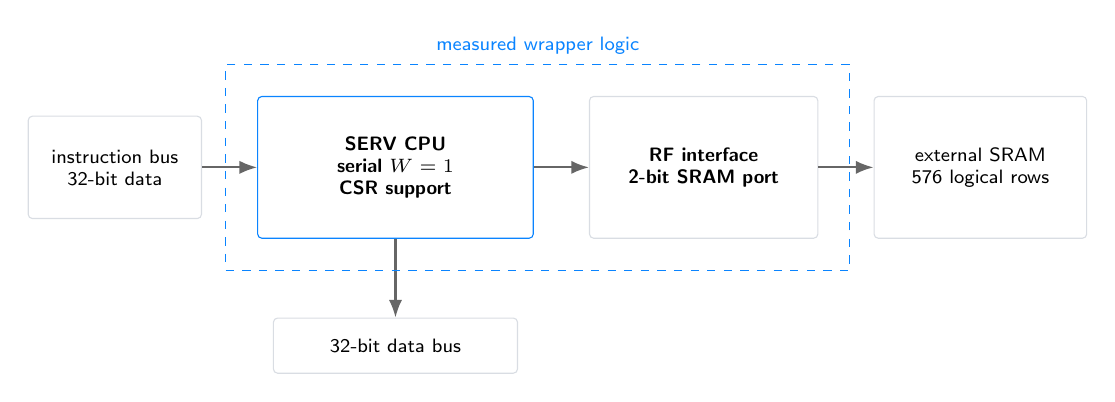
\begin{tikzpicture}[node distance=7mm]
\node[input,minimum width=22mm,minimum height=13mm] (ibus) {instruction bus\\32-bit data};
\node[accepted,right=of ibus,minimum width=35mm,minimum height=18mm] (cpu) {SERV CPU\\serial $W=1$\\CSR support};
\node[gate,right=of cpu,minimum width=29mm,minimum height=18mm] (rf) {RF interface\\2-bit SRAM port};
\node[input,right=of rf,minimum width=27mm,minimum height=18mm] (ram) {external SRAM\\576 logical rows};
\node[input,below=10mm of cpu,minimum width=31mm] (dbus) {32-bit data bus};
\draw[signal] (ibus)--(cpu);\draw[signal] (cpu)--(rf);\draw[signal] (rf)--(ram);\draw[signal] (cpu)--(dbus);
\node[draw=GotherBlue,dashed,fit=(cpu)(rf),inner sep=4mm,label={[font=\scriptsize,text=GotherBlue]above:measured wrapper logic}] {};
\end{tikzpicture}\end{center}

Instruction/data addresses, data, byte selects, cycle/write controls and acknowledgements retain the same comparison boundary. The SRAM read input and write/address outputs also remain fixed. No instruction or data memory is added to the measured design. Formal equivalence of this boundary is distinct from a complete ISA-compliance or system-validation campaign.

{\small\rowcolors{2}{Pale}{white}
\begin{tabularx}{\textwidth}{@{}Y P{37mm}P{37mm}@{}}
\rowcolor{Ink}\thead{Quantity} & \thead{Baseline} & \thead{Candidate} \\
GPR slots / RAM-backed CSR words & 32 / 4 & 32 / 4 \\
Word width / serial processing width & 32 bits / 1 bit & 32 bits / 1 bit \\
Logical register storage & 1,152 bits / 144 bytes & unchanged \\
SRAM row width / logical row count & 2 bits / 576 & unchanged \\
SRAM address-port width & 10 bits & unchanged \\
Mapped wrapper CLBs / flip-flops & 46 / 181 & 43 / 181 \\
\end{tabularx}\rowcolors{2}{}{}
}
\par
The four external CSR words are \texttt{mtvec}, \texttt{mscratch}, \texttt{mepc} and \texttt{mtval}. Other CSR state is held in wrapper logic. Capacity follows $(32+4)\times32=1{,}152$ bits, or $1{,}152/2=576$ logical rows. Ten address bits can encode more rows than this configured requirement; they do not establish additional allocated capacity.

\begin{scopebox}\textbf{Area boundary.} External SRAM area is excluded. The 181 mapped flip-flops describe wrapper state, not the 1,152-bit register-storage requirement. MWTA is VTR's minimum-width-transistor-area unit, not square millimetres.\end{scopebox}

% Page 4.
\newpageheading{3. Evaluation contract and sample}{Frozen before the final measurements}
The candidate is the development leader \nolinkurl{v2-exact-rf-high3-v2-lean-word-binary-m0}. Its eighteen-file tree is frozen by SHA-256. The final sample compares that one implementation with the original baseline; it does not select another candidate using final-seed outcomes.

{\small\rowcolors{2}{Pale}{white}
\begin{tabularx}{\textwidth}{@{}P{39mm}Y@{}}
\rowcolor{Ink}\thead{Dimension} & \thead{Frozen choice} \\
Interface and top & \texttt{serv\_synth\_wrapper}; all original public ports and cycle timing. \\
Configuration & \texttt{PRE\_REGISTER=1}, \texttt{RESET\_STRATEGY=MINI}, \texttt{WITH\_CSR=1}, \texttt{RF\_WIDTH=2}, \texttt{W=1}; MDU, compressed instructions and alignment extension disabled. \\
Implementation model & VTR commit \texttt{95f5c6de...}; homogeneous LUT6 target; PTM45 at 0.9 V and $85\,^{\circ}$C. \\
Activity & ACE static probability 0.5, input switching probability 0.2, clock probability 0.2; ACE seed 1. \\
Primary objective & Equal-weight geometric mean of paired total-area, routed-delay and active-total-power ratios. \\
Development guards & Area and power geometric ratios no greater than 1; source and mapped correctness mandatory. \\
Confirmatory rule & Composite one-sided 95\% upper ratio below 1 and no primary metric with one-sided lower ratio above 1. \\
Original editorial goal & Point score and one-sided upper score strictly below 0.90; multiplicity handling when applicable. \\
\end{tabularx}\rowcolors{2}{}{}
}
\par
\vspace{4mm}
{\small\rowcolors{2}{Pale}{white}
\begin{tabularx}{\textwidth}{@{}P{34mm}P{38mm}Y@{}}
\rowcolor{Ink}\thead{Sample} & \thead{Pair identities} & \thead{Status and role} \\
Development & 5001--5012 & 12 pairs, observed during selection; \textbf{3.4516\%} composite improvement. \\
Separate certification & 5101--5112 & Reserved twelve-pair gate, unexecuted for this candidate. \\
This fixed sample & 6001--6064 & \textbf{64 complete pairs / 128 fresh implementations}, prospectively registered before the first final run. \\
\end{tabularx}\rowcolors{2}{}{}
}
\par
The complete fixed sample is analysed once. It is not extended after inspection, pooled with development data or filtered to remove inconvenient placements. Pair identities match between both legs. Final measurements are separate from the earlier search and from two historical exploratory replicas under an older synthesis flow.

\begin{claimbox}\textbf{Decision.} The composite improves, but the delay lower confidence bound is \DelayLowerOneSidedRatio{}, above 1. The paired decision is \texttt{evidence\_regression}. The separate certification sample is still unused, and the strict greater-than-10\% editorial goal is not met.\end{claimbox}

% Page 5.
\newpageheading{4. Verification before measurement}{Recorded source and actual measured-state obligations}
Correctness is a prerequisite for interpreting any PPA result. The saved source gates check the exact baseline and candidate hashes. The adopted revision-2 flow also checks each RTL design against the BLIF netlist actually supplied to VPR, avoiding reliance on source-to-source equivalence alone.

{\small\rowcolors{2}{Pale}{white}
\begin{tabularx}{\textwidth}{@{}P{38mm}Y P{22mm}@{}}
\rowcolor{Ink}\thead{Gate} & \thead{Recorded evidence} & \thead{Result} \\
Syntax and hierarchy & Exact eighteen-file set and top; Verilator lint at serial widths 1 and 4. & \yes \\
Structural policy & Reject UNDRIVEN, MULTIDRIVEN and UNOPTFLAT warnings before implementation. & \yes \\
Source equivalence & Yosys \texttt{equiv\_simple} plus \texttt{equiv\_induct -undef}; 357 proved, zero unproved obligations per design. & \yes \\
Mapped equivalence & 126 primary output bits plus all 181 actual state bits: 307 proved / zero unproved for each design. & \yes \\
State binding & All original candidate FF bits bound once; unrelated internal-name matches disabled; undefined initialization preserved. & \yes \\
Mapped simulation & Two 4,096-cycle banks per design; each defined RTL output bit compared. Unknown RTL bits skipped. & \yes \\
Final record audit & All 128 report sets, source identities, netlist identities and paired metric rows checked. & \yes \\
PPA acceptance & Statistically supported primary timing regression. & \worse \\
\end{tabularx}\rowcolors{2}{}{}
}
\par
\begin{center}
\begin{tikzpicture}[node distance=6mm]
\node[input,minimum width=27mm] (src) {frozen RTL};
\node[gate,right=of src,minimum width=32mm] (gate) {source + mapped\\correctness};
\node[accepted,right=of gate,minimum width=28mm] (measure) {128 fixed\\implementations};
\node[gate,right=of measure,minimum width=31mm] (audit) {record audit\\then statistics};
\draw[signal](src)--(gate);\draw[signal](gate)--(measure);\draw[signal](measure)--(audit);
\end{tikzpicture}\end{center}

The source proof uses five-step simple equivalence and induction configured up to 80 steps; induction closure is not an 80-cycle-only simulation claim. The mapped proof adds demonstrated state correspondences rather than treating them as assumptions. It does not force undefined initial registers to zero. The simulation banks provide additional diagnostics, with their defined-bit limitation stated explicitly.

A mapped proof is reused across placement seeds only when both RTL identities match and every ordered executable BLIF statement has the same SHA-256 identity. Raw file hashes remain recorded; ABC timestamp comments may differ. Any executable netlist change requires another complete proof. The final audit verifies this reuse condition for every measured leg.

\begin{scopebox}\textbf{Trust scope.} These are saved project-operated equivalence records and audited implementations. Lint at $W=4$ does not establish a $W=4$ PPA result. Neither the formal record nor the consistency verifier is an external assurance opinion or full RISC-V ISA certification.\end{scopebox}

% Page 6.
\newpageheading{5. Exact source-change inventory}{One frozen combined candidate, ten edited files}
Both RTL trees contain eighteen files. The baseline has 3,562 total lines and 108,220 bytes; the candidate has 4,137 lines and 144,460 bytes. These totals include comments, blank lines and inactive parameter alternatives. The mapped area reduction is measured independently of source size.

{\small\rowcolors{2}{Pale}{white}
\begin{tabularx}{\textwidth}{@{}P{38mm}P{21mm}Y@{}}
\rowcolor{Ink}\thead{Edited file} & \thead{Lines B / C} & \thead{Change represented in the frozen tree} \\
\texttt{serv\_rf\_ram\_if.v} & 186 / 344 & Split low/high phase and explicit read/write phase views. \\
\texttt{serv\_decode.v} & 367 / 556 & Encoded instruction fields, decode rewrites and selectable capture usage. \\
\texttt{serv\_bufreg.v} & 101 / 232 & Reversible address-state representation and logical data view. \\
\texttt{serv\_bufreg2.v} & 105 / 163 & Factored byte/shift/count controls and word-enable form. \\
\texttt{serv\_ctrl.v} & 115 / 129 & Selected PC word-enable and reset-priority expression. \\
\texttt{serv\_alu.v} & 87 / 90 & Result selection expressed as a priority structure. \\
\texttt{serv\_csr.v} & 164 / 175 & Factored CSR cause update terms. \\
\texttt{serv\_state.v} & 239 / 239 & Local control-expression rewrites. \\
\texttt{serv\_top.v} & 674 / 680 & Parameter plumbing into the selected module forms. \\
\texttt{serv\_synth\_wrapper.v} & 138 / 143 & Frozen selectors defining the measured configuration. \\
\end{tabularx}\rowcolors{2}{}{}
}
\par
\subsection{The wrapper fixes the measured path}
\begin{lstlisting}[language=VerilogDiff]
RF_HIGH_PHASE_FORM        = 1
DECODER_CAPTURE_USAGE_FORM = 3
PC_WORD_ENABLE_FORM        = 3
DATA_WORD_ENABLE_FORM      = 3
BUFFER_CONTROL_FORM       = 3
\end{lstlisting}
These are parameter selections, not five separately measured contributions. In particular, decoder usage form 3 selects the original \texttt{ALU\_sub} and \texttt{RD\_op} expressions; the candidate cannot be described as gaining from active registered substitutes for those two signals.

The exact unified patch is preserved at \texttt{rtl/changes.patch}. The next three pages explain active structural views with verified source references. The complete patch includes alternatives compiled out by the fixed wrapper and is therefore kept as a machine-verifiable artifact rather than reproducing every inactive branch in this fourteen-page report.

\begin{scopebox}\textbf{Attribution limit.} The 64 pairs measure the entire combined candidate. No isolated percentage is assigned to an individual file, encoding or structural view. Identifying the source of a PPA consequence requires controlled comparisons under a new frozen experiment.\end{scopebox}

% Page 7.
\newpageheading{6. Structural view 1: register-file phase}{Source: serv\_rf\_ram\_if.v:103--128 and 224--238; form 1}
The baseline stores a five-bit serial counter for $W=1$. Its write position is expressed as \texttt{wcnt = rcnt - 4}. The candidate separates a two-bit low counter from a three-bit physical high phase. A decoded four-bit logical phase supplies the existing high read-count and write-count views; it is not a fourth stored phase bit in the selected form.

\begin{center}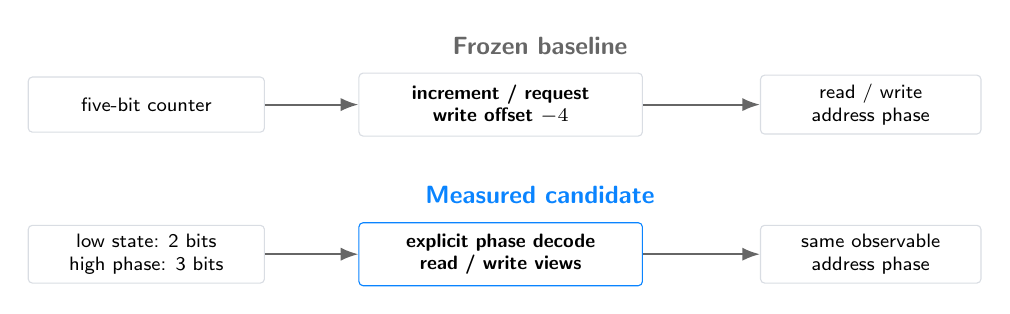
\begin{tikzpicture}
\node[font=\small\bfseries,text=Mid] at (0,1.2) {Frozen baseline};
\node[input,minimum width=30mm] (b) at (-5,0.45) {five-bit counter};
\node[gate,minimum width=36mm] (bm) at (-.5,.45) {increment / request\\write offset $-4$};
\node[input,minimum width=28mm] (bo) at (4.2,.45) {read / write\\address phase};
\draw[signal](b)--(bm);\draw[signal](bm)--(bo);
\node[font=\small\bfseries,text=GotherBlue] at (0,-.7) {Measured candidate};
\node[input,minimum width=30mm] (a) at (-5,-1.45) {low state: 2 bits\\high phase: 3 bits};
\node[accepted,minimum width=36mm] (am) at (-.5,-1.45) {explicit phase decode\\read / write views};
\node[input,minimum width=28mm] (ao) at (4.2,-1.45) {same observable\\address phase};
\draw[signal](a)--(am);\draw[signal](am)--(ao);
\end{tikzpicture}\end{center}

For binary phase bits $p_2,p_1,p_0$, selected form 1 reconstructs the four-bit logical phase $h$ as
\[
\begin{aligned}
h_0&=p_0\oplus p_1\oplus(p_0p_1)\oplus p_2,& h_1&=p_1\oplus p_2,\\
h_2&=(p_0p_1)\oplus p_2,& h_3&=p_2.
\end{aligned}
\]
The existing read view $\{h_3,h_3\oplus h_1,\bigoplus h\}$ simplifies to $\{p_2,p_1,p_0\}$. The write view represents the high-field offset associated with subtracting four from the complete serial counter. This distributes the arithmetic into explicit Boolean views while preserving the original observable sequence.

{\small\rowcolors{2}{Pale}{white}
\begin{tabularx}{\textwidth}{@{}P{31mm}Y P{39mm}@{}}
\rowcolor{Ink}\thead{Binary high phase} & \thead{Decoded logical phase $h_3h_2h_1h_0$} & \thead{Next high phase} \\
0, 1, 2, 3 & 0000, 0001, 0011, 0111 & 1, 2, 3, 4 \\
4, 5, 6, 7 & 1111, 1110, 1100, 1000 & 5, 6, 7, 0 \\
\end{tabularx}\rowcolors{2}{}{}
}
\par
The high phase advances when both low bits are one. Request handling loads the original low-count value and resets the high phase; minimal reset retains the original assignment priority. Other serial widths use the fallback binary path. No PPA claim is made for those widths.

\begin{claimbox}\textbf{Measured consequence.} The whole wrapper still uses 181 flip-flops. Its CLB count falls from 46 to 43, but the complete candidate's delay increases. This representation is one part of the measured combination; its separate timing or power contribution is not established.\end{claimbox}

% Page 8.
\newpageheading{7. Structural view 2: instruction decode}{Source: serv\_decode.v:423--438; wrapper usage form 3}
With \texttt{PRE\_REGISTER=1}, instruction fields are retained at the instruction-data capture edge and used by later decode logic. The candidate changes selected field representations and Boolean cones while preserving the instruction interface and update enable. One visible recoding stores \texttt{funct3} with polarity mask \texttt{3'b101}; a logical view reconstructs its meaning.

\begin{center}
\begin{tikzpicture}[node distance=8mm]
\node[input,minimum width=28mm] (in) {instruction data};
\node[gate,right=of in,minimum width=34mm] (reg) {field capture\\\texttt{i\_wb\_en}};
\node[accepted,right=of reg,minimum width=34mm] (logic) {logical field views\\factored decoder};
\node[input,right=of logic,minimum width=26mm] (out) {same cycle\\control outputs};
\draw[signal](in)--(reg);\draw[signal](reg)--(logic);\draw[signal](logic)--(out);
\end{tikzpicture}\end{center}

\subsection{What usage form 3 actually selects}
\begin{lstlisting}[language=VerilogDiff,basicstyle=\ttfamily\scriptsize,breaklines=true]
assign co_alu_sub =
  (CAPTURE_USAGE_FORM == 2 || CAPTURE_USAGE_FORM == 3)
  ? legacy_co_alu_sub : captured_alu_sub;
assign co_rd_op =
  (CAPTURE_USAGE_FORM == 1 || CAPTURE_USAGE_FORM == 3)
  ? legacy_co_rd_op : captured_rd_op;
// Selected wrapper: CAPTURE_USAGE_FORM = 3
\end{lstlisting}
Both outputs therefore use their original Boolean expressions in the measured configuration. The source still declares and updates captured substitutes for alternative modes. Their presence in the file does not prove that they contribute physical state or an improvement in this selected netlist; synthesis can remove unused paths.

\subsection{Other local control rewrites}
The ALU result expression selects comparison, addition or Boolean results with a priority structure before combining with the buffer input. The source comment refers to mutually exclusive selects produced by the decoder; this report relies on integrated-core equivalence rather than adding an independent one-hot premise. CSR cause updates also expose shared interrupt/event terms, with clocked update priority retained.

The decoder's field polarity, selected result structure and shared control terms can change LUT mapping and fanout even when the logical machine is equivalent. Source-level simplification alone does not guarantee a shorter routed critical path. The final 64-pair result is the relevant implementation evidence for this target.

\begin{scopebox}\textbf{Timing interpretation.} Equivalent cycle behaviour means the same logical state and outputs at the comparison boundary. It does not mean equal physical propagation delay. A cycle-equivalent rewrite can be smaller and lower-power while mapping to a slower routed path, as observed here.\end{scopebox}

% Page 9.
\newpageheading{8. Structural view 3: buffers and PC}{Source: serv\_bufreg.v:65--80 and 161--162; serv\_ctrl.v:124--125}
The address buffer retains 32 physical bits but changes how some of them encode the logical address. For positions 12--15, a prefix-XOR logical view reconstructs four original data bits. A further reversible shear affects physical bit 14 using neighbouring bits. Positions 18/19 and 24/25 also use paired coordinates. Other bit positions preserve their direct view.

\begin{center}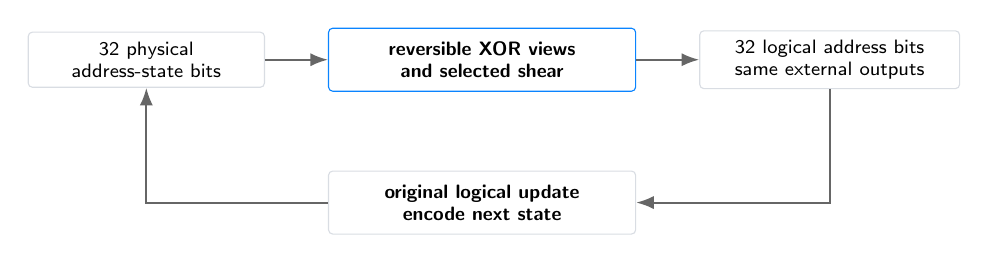
\begin{tikzpicture}[node distance=8mm]
\node[input,minimum width=30mm] (physical) {32 physical\\address-state bits};
\node[accepted,right=of physical,minimum width=39mm] (decode) {reversible XOR views\\and selected shear};
\node[input,right=of decode,minimum width=33mm] (logical) {32 logical address bits\\same external outputs};
\draw[signal](physical)--(decode);\draw[signal](decode)--(logical);
\node[gate,below=10mm of decode,minimum width=39mm] (next) {original logical update\\encode next state};
\draw[signal](logical.south)|-(next.east);\draw[signal](next.west)-|(physical.south);
\end{tikzpicture}\end{center}
If $a$ denotes the intermediate address code, the illustrated prefix view is
\[
\begin{aligned}
d_{12}&=a_{12}\oplus a_{13}\oplus a_{14}\oplus a_{15},&d_{13}&=a_{13}\oplus a_{14}\oplus a_{15},\\
d_{14}&=a_{14}\oplus a_{15},&d_{15}&=a_{15}.
\end{aligned}
\]
The next logical address is encoded before writing physical state. For binary values the XOR map is invertible, and the shear $a_{14}=p_{14}\oplus(p_{13}p_{15})$ is its own inverse when its control bits are retained. These equations explain the representation; the recorded sequential proof establishes the frozen core's equivalence scope.

\subsection{Word banks preserve priority, not just truth tables}
The selected data-buffer form factors byte-valid, shift and count conditions. Word-enable form 3 explicitly preserves load-versus-shift selection. The PC form similarly retains reset priority at the same active clock edge:
\begin{lstlisting}[language=VerilogDiff,basicstyle=\ttfamily\scriptsize]
if (i_rst | i_pc_en)
  o_ibus_adr <= i_pc_en
    ? (i_rst ? RESET_PC : {new_pc,o_ibus_adr[31:W]})
    : RESET_PC;
\end{lstlisting}
When neither reset nor PC enable is active, the register holds. When both are active, reset still determines the loaded value. No added pipeline stage, clock change, larger memory or interface-latency change is introduced by this expression.

\begin{claimbox}\textbf{Evidence boundary.} State representation and update-expression changes are evaluated as one frozen candidate. The unchanged 181-FF total does not imply unchanged logic cones, routing or maximum clock estimate. The timing regression remains a real implementation consequence.\end{claimbox}

% Page 10.
\newpageheading{9. PPA environment, flow repair and statistics}{Pinned academic model; paired implementation variability}
The implementation target is VTR's homogeneous \texttt{k6\_N10\_I40\_Fi6\_L4\_frac0\_ff1\_45nm} architecture: six-input LUTs, ten per clustered logic block, with the target's routing and timing model. PTM45 supplies technology properties at 0.9 V and $85\,^{\circ}$C. Baseline and candidate use the same placement seed, activity model, wrapper configuration and tool image in each pair.

\subsection{The common subtraction-lowering repair}
An earlier flow showed a discrepancy between source RTL and a measured mapped implementation. Revision 2 expands subtraction through the standard Yosys Boolean map before Parmys, then checks that no \texttt{\$sub} cell remains. This repair is applied to both legs. Actual RTL-to-measured-netlist proof is required; a favourable source-level score cannot excuse incorrect mapping.
\begin{lstlisting}[basicstyle=\ttfamily\scriptsize]
techmap -map +/techmap.v {t:$sub}
opt -full
select -assert-none {t:$sub}
\end{lstlisting}
Historical gains from the older flow are not pooled into this sample. The pinned image is \nolinkurl{serv-study-vtr-ppa45:20261005}; its exact image ID, VTR commit, synthesis-template hash and source identities are recorded in the evidence package.

\subsection{Estimator and interval definitions}
For metric $m$ and pair $p$, $\ell_{m,p}=\log(M_{C,m,p}/M_{B,m,p})$. With $A$ total area, $D$ post-route delay and $P$ active total power,
\[
r_p=\sqrt[3]{r_{A,p}r_{D,p}r_{P,p}},\qquad
\widehat r=\exp\!\left(\frac{1}{64}\sum_{p=1}^{64}\log r_p\right).
\]
Two-sided display intervals are $\exp(\bar\ell\pm t_{0.975,63}s_\ell/8)$, with $t=1.9983405425$. Improvement is $100(1-r)$, so negative timing improvement means greater delay. The acceptance rule uses the separately declared one-sided critical $t_{0.95,63}=1.6694022217$.

\begin{scopebox}\textbf{Acceptance result.} The composite one-sided upper ratio is \UpperOneSidedScore{}, below 1. However, the delay one-sided lower ratio is \DelayLowerOneSidedRatio{}, above 1: primary timing regression is supported. The strict 0.90 editorial score threshold also fails. A positive composite does not override either condition.\end{scopebox}

ACE activity is probabilistic, not an application execution trace. Power and area are model estimates. These intervals quantify variability across the fixed implementation seeds; they do not cover silicon PVT distributions, workload uncertainty, tool drift or external-memory energy. Reciprocal delay is reported only as a frequency estimate, not as measured CPU throughput.

% Page 11.
\newpageheading{10. Every fixed paired result}{All 64 baseline and candidate placements}
\begin{center}\begin{tikzpicture}
\begin{axis}[width=.94\textwidth,height=105mm,xmin=\CloudMin,xmax=\CloudMax,ymin=.65,ymax=4.65,
 ytick={1,2,3,4},yticklabels={Area,Timing,Active power,Composite},
 xtick distance=5,xticklabel={\pgfmathprintnumber{\tick}\%},
 xlabel={Improvement relative to the same baseline aggregate (right is better)},
 grid=major,grid style={draw=Rule},axis line style={draw=Mid},tick label style={font=\small},label style={font=\small\bfseries},
 legend style={at={(0.5,1.03)},anchor=south,draw=none,font=\footnotesize,legend columns=-1}]
\addplot[only marks,mark=*,mark size=1.35pt,Mid,opacity=.28] table[x=baseline_area,y expr=1+0.46*\thisrow{jitter},col sep=comma]{generated/pair-clouds.csv};
\addlegendentry{Baseline pairs}
\addplot[only marks,mark=*,mark size=1.35pt,GotherBlue,opacity=.38] table[x=optimized_area,y expr=1+0.46*\thisrow{jitter},col sep=comma]{generated/pair-clouds.csv};
\addlegendentry{Candidate pairs}
\foreach \metric/\level in {timing/2,power/3,composite/4}{
\addplot[only marks,mark=*,mark size=1.35pt,Mid,opacity=.28,forget plot] table[x=baseline_\metric,y expr=\level+0.46*\thisrow{jitter},col sep=comma]{generated/pair-clouds.csv};
\addplot[only marks,mark=*,mark size=1.35pt,GotherBlue,opacity=.38,forget plot] table[x=optimized_\metric,y expr=\level+0.46*\thisrow{jitter},col sep=comma]{generated/pair-clouds.csv};}
\addlegendimage{line legend,Ink,line width=1pt,mark=*,mark size=1.4pt}\addlegendentry{Paired estimate and 95\% CI}
\draw[Ink,line width=1pt](axis cs:\AreaLow,1.23)--(axis cs:\AreaHigh,1.23);\fill[Ink](axis cs:\AreaImprovement,1.23)circle[radius=1.8pt];
\draw[Regress,line width=1.3pt](axis cs:\DelayLow,2.23)--(axis cs:\DelayHigh,2.23);\fill[Regress](axis cs:\DelayImprovement,2.23)circle[radius=2pt];
\draw[Ink,line width=1pt](axis cs:\PowerLow,3.23)--(axis cs:\PowerHigh,3.23);\fill[Ink](axis cs:\PowerImprovement,3.23)circle[radius=1.8pt];
\draw[Ink,line width=1pt](axis cs:\CompositeLow,4.23)--(axis cs:\CompositeHigh,4.23);\fill[Ink](axis cs:\CompositeImprovement,4.23)circle[radius=1.8pt];
\draw[Ink,line width=1.1pt](axis cs:0,.65)--(axis cs:0,4.65);
\end{axis}\end{tikzpicture}\end{center}
\smallcaps{Figure 2 · Complete pair clouds and paired log-ratio intervals}\par
Points are absolute implementations normalized to the same baseline geometric aggregate. Both legs of a pair receive identical vertical jitter. Interval marks use paired ratios, so their position need not match a raw cloud's centre. All 64 pairs are included; the red timing interval lies entirely on the regression side of zero.

{\small\rowcolors{2}{Pale}{white}
\begin{tabularx}{\textwidth}{@{}Y R R R@{}}
\rowcolor{Ink}\thead{Metric} & \thead{Wins} & \thead{Ties} & \thead{Losses} \\
Area & \AreaWins & \AreaTies & \AreaLosses \\
Timing & \DelayWins & \DelayTies & \textcolor{Regress}{\DelayLosses} \\
Active power & \PowerWins & \PowerTies & \PowerLosses \\
Composite & \CompositeWins & \CompositeTies & \CompositeLosses \\
\end{tabularx}\rowcolors{2}{}{}
}
\par
\vspace{3mm}
\begin{claimbox}\textbf{Result.} A composite win in every pair coexists with timing losses in 48 pairs. The primary-metric guard makes this combination ineligible for acceptance under the frozen rule.\end{claimbox}

% Page 12: include every pair numerically, not just as a cloud.
\newpageheading{11. All 64 paired measurements}{Compact numerical ledger, no omitted placements}
Every number below is an improvement percentage $100(1-M_C/M_B)$ for the matched pair. A, D and P denote area, delay and power; C is the equal-weight per-pair composite. \textcolor{Regress}{Negative timing values mean higher delay} and are highlighted. The full-precision ratios, absolute metrics and source hashes are retained in \nolinkurl{results/confirmation64.json}; rounding here does not change the estimator.
\par\vspace{4mm}\noindent
\begin{minipage}[t]{.485\textwidth}
{\scriptsize\renewcommand{\arraystretch}{1.36}\rowcolors{2}{Pale}{white}
\begin{tabularx}{\linewidth}{@{}r R R R R@{}}
\rowcolor{Ink}\thead{Seed} & \thead{A \%} & \thead{D \%} & \thead{P \%} & \thead{C \%} \\
6001 & 5.891 & \textcolor{Regress}{-1.069} & 7.218 & 4.081 \\
6002 & 5.891 & \textcolor{Regress}{-7.498} & 8.843 & 2.664 \\
6003 & 5.891 & \textcolor{Regress}{-4.726} & 7.048 & 2.879 \\
6004 & 5.891 & 1.453 & 3.635 & 3.677 \\
6005 & 5.891 & \textcolor{Regress}{-7.802} & 9.255 & 2.719 \\
6006 & 5.891 & \textcolor{Regress}{-0.795} & 4.649 & 3.291 \\
6007 & 5.891 & \textcolor{Regress}{-10.000} & 9.662 & 2.209 \\
6008 & 5.891 & 3.064 & 2.446 & 3.812 \\
6009 & 5.891 & \textcolor{Regress}{-0.709} & 5.584 & 3.636 \\
6010 & 6.518 & \textcolor{Regress}{-5.896} & 10.599 & 3.990 \\
6011 & 6.518 & \textcolor{Regress}{-3.444} & 10.173 & 4.586 \\
6012 & 5.891 & \textcolor{Regress}{-1.665} & 6.109 & 3.511 \\
6013 & 5.891 & 2.683 & 2.873 & 3.827 \\
6014 & 5.576 & 2.243 & 2.477 & 3.444 \\
6015 & 5.891 & \textcolor{Regress}{-2.854} & 6.060 & 3.120 \\
6016 & 5.297 & \textcolor{Regress}{-1.101} & 3.248 & 2.518 \\
6017 & 5.891 & \textcolor{Regress}{-3.985} & 6.283 & 2.843 \\
6018 & 5.891 & \textcolor{Regress}{-3.388} & 7.852 & 3.574 \\
6019 & 5.891 & \textcolor{Regress}{-0.785} & 4.578 & 3.271 \\
6020 & 6.518 & \textcolor{Regress}{-1.977} & 7.819 & 4.217 \\
6021 & 5.891 & \textcolor{Regress}{-4.945} & 8.125 & 3.188 \\
6022 & 5.891 & \textcolor{Regress}{-0.079} & 5.694 & 3.875 \\
6023 & 5.891 & \textcolor{Regress}{-2.584} & 6.921 & 3.502 \\
6024 & 5.891 & 0.346 & 5.103 & 3.811 \\
6025 & 5.891 & \textcolor{Regress}{-7.608} & 8.616 & 2.550 \\
6026 & 6.518 & 2.989 & 3.563 & 4.370 \\
6027 & 5.891 & \textcolor{Regress}{-3.088} & 6.875 & 3.328 \\
6028 & 5.297 & \textcolor{Regress}{-1.146} & 1.936 & 2.064 \\
6029 & 5.891 & \textcolor{Regress}{-6.026} & 9.288 & 3.268 \\
6030 & 5.891 & \textcolor{Regress}{-1.934} & 5.459 & 3.204 \\
6031 & 5.891 & 0.979 & 2.715 & 3.217 \\
6032 & 5.891 & 1.070 & 3.775 & 3.599 \\

\end{tabularx}\rowcolors{2}{}{} }
\end{minipage}\hfill
\begin{minipage}[t]{.485\textwidth}
{\scriptsize\renewcommand{\arraystretch}{1.36}\rowcolors{2}{Pale}{white}
\begin{tabularx}{\linewidth}{@{}r R R R R@{}}
\rowcolor{Ink}\thead{Seed} & \thead{A \%} & \thead{D \%} & \thead{P \%} & \thead{C \%} \\
6033 & 5.576 & 4.479 & 0.953 & 3.690 \\
6034 & 5.891 & \textcolor{Regress}{-2.839} & 7.855 & 3.746 \\
6035 & 5.891 & \textcolor{Regress}{-1.700} & 3.854 & 2.734 \\
6036 & 6.518 & \textcolor{Regress}{-4.986} & 10.720 & 4.309 \\
6037 & 5.891 & \textcolor{Regress}{-0.492} & 4.994 & 3.505 \\
6038 & 5.891 & \textcolor{Regress}{-0.634} & 5.467 & 3.620 \\
6039 & 5.891 & \textcolor{Regress}{-3.794} & 8.382 & 3.633 \\
6040 & 5.891 & \textcolor{Regress}{-0.995} & 4.001 & 3.009 \\
6041 & 5.297 & \textcolor{Regress}{-3.426} & 3.824 & 1.971 \\
6042 & 5.891 & 0.559 & 5.272 & 3.937 \\
6043 & 5.891 & 1.106 & 3.455 & 3.504 \\
6044 & 6.518 & 0.184 & 6.433 & 4.424 \\
6045 & 5.891 & \textcolor{Regress}{-7.795} & 8.963 & 2.617 \\
6046 & 5.576 & \textcolor{Regress}{-4.022} & 6.698 & 2.867 \\
6047 & 5.891 & \textcolor{Regress}{-5.296} & 10.116 & 3.785 \\
6048 & 5.891 & \textcolor{Regress}{-0.585} & 4.926 & 3.452 \\
6049 & 5.891 & \textcolor{Regress}{-3.451} & 5.190 & 2.634 \\
6050 & 5.891 & 4.109 & 1.152 & 3.737 \\
6051 & 5.891 & 5.442 & -0.291 & 3.721 \\
6052 & 5.891 & \textcolor{Regress}{-2.015} & 2.766 & 2.268 \\
6053 & 5.891 & \textcolor{Regress}{-0.580} & 5.080 & 3.506 \\
6054 & 5.891 & \textcolor{Regress}{-0.104} & 5.241 & 3.713 \\
6055 & 6.518 & \textcolor{Regress}{-5.173} & 9.127 & 3.686 \\
6056 & 5.891 & \textcolor{Regress}{-4.618} & 8.915 & 3.566 \\
6057 & 5.891 & \textcolor{Regress}{-6.348} & 9.675 & 3.308 \\
6058 & 5.576 & \textcolor{Regress}{-1.076} & 4.319 & 2.982 \\
6059 & 5.891 & \textcolor{Regress}{-1.817} & 4.560 & 2.935 \\
6060 & 5.891 & 0.207 & 6.630 & 4.285 \\
6061 & 5.891 & \textcolor{Regress}{-3.123} & 6.421 & 3.160 \\
6062 & 5.576 & \textcolor{Regress}{-8.974} & 9.046 & 2.184 \\
6063 & 5.891 & 0.530 & 4.190 & 3.563 \\
6064 & 5.297 & \textcolor{Regress}{-0.522} & 1.772 & 2.212 \\

\end{tabularx}\rowcolors{2}{}{} }
\end{minipage}
\par\vspace{5mm}
The reported \CompositeImprovement\% headline is computed from the mean of full-precision paired logs, not the average of these rounded percentages. The complete sequence is the prospectively reserved sample 6001--6064. No earlier development or exploratory-replica seed is substituted into this ledger.

% Page 13.
\newpageheading{12. Resources, evidence and reproduction}{Measured consequences and local audit trail}
{\small\rowcolors{2}{Pale}{white}
\begin{tabularx}{\textwidth}{@{}P{35mm}P{32mm}P{32mm}Y@{}}
\rowcolor{Ink}\thead{Quantity} & \thead{Baseline} & \thead{Candidate} & \thead{Interpretation} \\
Packed CLBs & 46 & 43 & 6.5217\% fewer in every pair. \\
Mapped flip-flops & 181 & 181 & Same wrapper-state count. \\
Delay-derived Fmax & \BaselineFmax\ MHz & \OptimizedFmax\ MHz & \textcolor{Regress}{\FmaxReduction\% lower}; not measured throughput. \\
External RF capacity & 1,152 bits & 1,152 bits & Same 576 logical two-bit rows; area excluded. \\
Development score & 1.000000 & 0.965484 & 3.4516\% on twelve selection pairs. \\
Fixed 64-pair score & 1.000000 & \CompositeScore & \CompositeImprovement\%; timing guard fails. \\
\end{tabularx}\rowcolors{2}{}{}
}
\par
The local evidence package contains both exact RTL trees, their unified patch, the original development records, correctness logs/models and the final 128 timing, power and measured-BLIF report sets. Each final result is tied to the selected source and the measured executable netlist. The full private search archive and optimizer are outside the report package.

{\small\rowcolors{2}{Pale}{white}
\begin{tabularx}{\textwidth}{@{}P{39mm}Y@{}}
\rowcolor{Ink}\thead{Evidence object} & \thead{SHA-256 identity} \\
Baseline RTL tree & \hash{\BaselineRtlHash} \\
Candidate RTL tree & \hash{\OptimizedRtlHash} \\
Audited 64-pair result & \hash{\FinalResultHash} \\
\end{tabularx}\rowcolors{2}{}{}
}
\par
\subsection{Consistency verification}
\begin{lstlisting}[basicstyle=\ttfamily\scriptsize]
# From the local repository root:
python3 experiments/serv-1.4.0/verify.py
python3 verify.py
\end{lstlisting}
The verifier checks exact source identities and the patch, saved formal closure markers and netlist identities, raw report extraction for each pair, all 64 ratios, confidence intervals and the rejected acceptance decision. Package checksums and fixed authorities bind the recorded evidence. Verification recomputes the saved result; it does not launch another EDA implementation or independently regenerate a proof.

\begin{scopebox}\textbf{Reproduction boundary.} A fresh run requires the exact Linux/amd64 image, VTR commit, architecture/PTM files, common synthesis repair, ACE activity contract and frozen RTL. A substituted library, clock/activity policy or integration is another experiment. This edition remains local; no GitHub upload or public release is asserted.\end{scopebox}

% Page 14.
\newpageheading{13. Search history, limits and conclusion}{A verified RTL candidate with an unacceptable timing trade-off}
The closed revision-2 search registered 2,812 candidates: 2,621 received valid PPA measurements and 191 were excluded without PPA. These are exploratory records, not independent acceptance trials. The RF-phase cohort had 36 measured candidates before the leader received its twelve-pair development comparison. Later searches combined changes on the leader and other promising parents; none of the completed validated combinations superseded it.

Historical numbers remain separate. An apparent 11.10461\% gain was rejected for mapping incoherence. A 4.4778\% result was not recertified after the common subtraction-lowering repair. Two older exploratory 64-pair replicas do not certify this candidate. The final unfinished branch/trap family prepared nine variants; three native banks passed, six remained pending and no PPA result was obtained for that family.

The user paused optimization after repeated storage stops, then requested this fixed 64-pair measurement of the preserved leader. The source was unchanged during that sample. This report replaces the earlier four-page development summary with the complete measured outcome and the same design system as the other portfolio reports.

\begin{claimbox}\textbf{Conclusion.} Area falls by \AreaImprovement\% and estimated active power by \PowerImprovement\%. The composite improves by \CompositeImprovement\%, but routed delay increases by \DelayIncrease\%, with a confidence interval entirely above no change. The frozen no-primary-regression rule rejects the candidate. The strict greater-than-10\% target is unmet, and the separate twelve-pair certification sample remains unused.\end{claimbox}

The equivalence records support the configured RTL boundary. They do not establish ISA certification, a signed external assurance opinion, ASIC signoff, commercial-FPGA performance, manufactured-silicon behaviour, measured board power or application energy. The academic homogeneous LUT6 model does not represent the external SRAM's physical area or energy. Cross-case percentages are not a performance ranking of unlike circuits.

No single source rewrite is proven responsible for the timing regression. Identifying a contributor requires new controlled comparisons with the same correctness, target and activity boundaries. Publication as an accepted case would require satisfying the actual acceptance rules; changing a label cannot remove the measured trade-off. The next technical decision is whether to investigate timing further under a separately frozen experiment.

\subsection{Source, licensing and primary references}
{\small
\begin{itemize}
\item \href{https://github.com/olofk/serv/tree/7d9cde4e6ca4f4c84d7512a752a4c187537dd373/rtl}{SERV 1.4.0 RTL at the pinned upstream commit}. Original ISC headers and license are retained.
\item \href{https://github.com/verilog-to-routing/vtr-verilog-to-routing/tree/95f5c6de9e158371ba7185bf97c07a84153735d6}{Pinned VTR source}. The derived synthesis template retains the bundled upstream terms.
\item Local \texttt{contract.json}, \texttt{provenance.json}, \texttt{results/confirmation64.json}, \texttt{rtl/changes.patch} and the saved evidence verifier.
\end{itemize}
}
Original Göther Labs presentation and verification work follows the repository MIT license. SERV, its contributors and tool providers do not endorse this study.
\end{document}
